\section{Обработка табличных данных. Часть 1 }

\subsection{Условие задания}
Создать приложение для выполнения задания. Использовать элемент формы DataGridView. 

\textbf{ДИАПАЗОН [a,b] означает, что mas[i][j] >= a \&\& mas[i][j] <= b.}

Приложение должно выполнять следующие действия:

\begin{enumerate}
    \item Возможность удалять и добавлять строки таблицы. Проект не должен аварийно завершаться при удалении несуществующей таблицы.
    \item Проверять ввод не числовых данных как в таблицу, так и в остальные текстовые поля (если есть в задании).
    \item Если есть диапазон значений [a,b], проверять, что a < b.
    \item Заголовок формы должен отражать суть задания.
    \item Все элементы формы должны быть внятно подписаны (кнопки подписаны, у тестового поля должно быть написано, для чего оно нужно и т. д.)
    \item В коде должны быть комментарии и отступы (код должен быть легко читаем).
    \item В коде программы все элементы формы должны быть переименованы (btnName -  для кнопок, lblName - для ссылок, txtName - для текстового поля и т. д.) Наименования должны быть понятными.
    \item Приложение должно корректно работать (выводить ответ или ошибку с соответствующим сообщением). После вывода ошибок при вводе корректных данных поля ошибок должны очищаться.  
\end{enumerate}

\textbf{Вариант 9.} Смотреть на рисунке \ref{task4_var9}.
\begin{figure}[H]
    \centering
    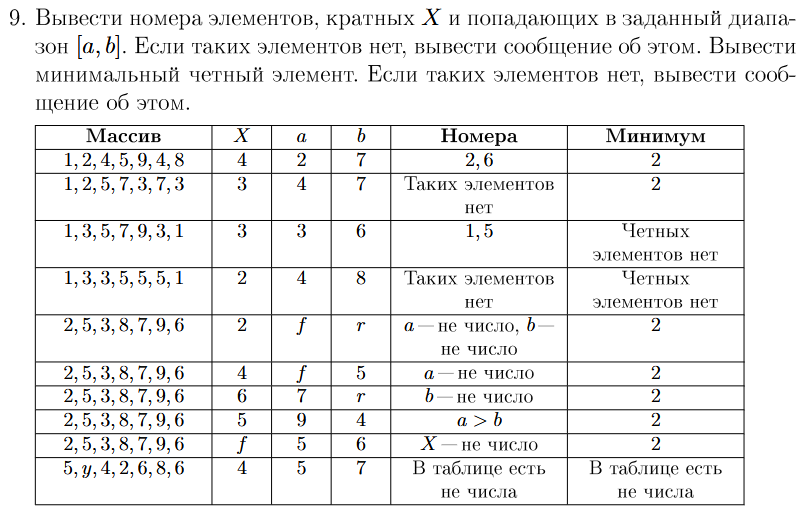
\includegraphics[width=0.9\linewidth]{lections/img/task4_var9.png}
    \caption{Задание 4 Вариант 9}
    \label{task4_var9}
\end{figure}

\subsection{Вид формы в конструкторе}

Создано окно приложения, содержащее пять элементов TextBox, четыре элемента Label, четыре элемента Button, один элемент gridview и один элемент ErrorProvider для обработки ошибок. Вид окна представлен на рисунке \ref{task4_form} \cite{ахо2000структуры}.
\begin{figure}[H]
    \centering
    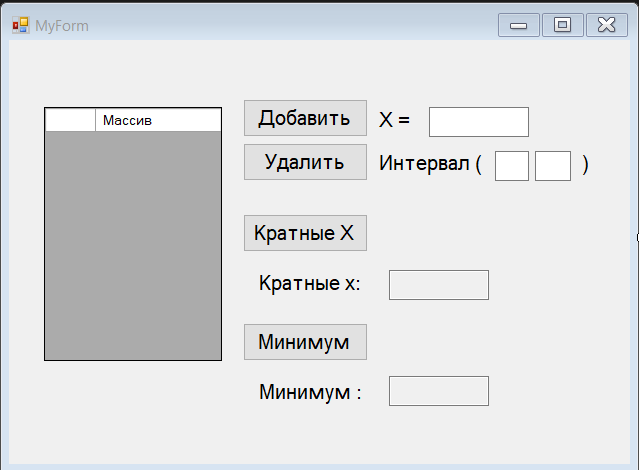
\includegraphics[width=0.8\linewidth]{lections/img/task4_form.png}
    \caption{Окно приложения «Обработка табличных данных. Часть 1» открытое в конструкторе}
    \label{task4_form}
\end{figure}


\subsection{Таблица с описанием переименованных элементов формы}
Все измененные элементы формы указаны в таблице \ref{task4_attributes}.


\begin{table}[H]
\caption{Значения атрибутов элементов в приложении <<Обработка табличных данных. Часть 1>>}
\begin{tabular}{|l|l|l|}
\hline
\textbf{\begin{tabular}[c]{@{}l@{}}Описание элементов\\ формы\end{tabular}} & \textbf{\begin{tabular}[c]{@{}l@{}}Список измененных\\ атрибутов\end{tabular}} & \textbf{\begin{tabular}[c]{@{}l@{}}Новое значение\\ атрибута\end{tabular}}    \\ \hline
Форма MyForm                                                                & Text                                                                           & \begin{tabular}[c]{@{}l@{}}Обработка табличных\\ данных. Часть 1\end{tabular} \\ \hline
TextBox ввода X                                                             & Name                                                                           & x\_input                                                                      \\ \hline
TextBox ввода начала интервала                                              & Name                                                                           & int\_a                                                                        \\ \hline
TextBox ввода конца интервала                                               & Name                                                                           & int\_b                                                                        \\ \hline
\multirow{2}{*}{TextBox вывода кратных х}                                   & Name                                                                           & krat\_box                                                                     \\ \cline{2-3} 
                                                                            & ReadOnly                                                                       & True                                                                          \\ \hline
\multirow{2}{*}{TextBox вывода минимума}                                    & Name                                                                           & chet\_box                                                                     \\ \cline{2-3} 
                                                                            & ReadOnly                                                                       & True                                                                          \\ \hline
Кнопка "Добавить"                                                           & Name                                                                           & mas\_add                                                                      \\ \hline
                                                                            & Text                                                                           & Добавить                                                                      \\ \hline
\multirow{2}{*}{Кнопка "Удалить"}                                           & Name                                                                           & mas\_pop                                                                      \\ \cline{2-3} 
                                                                            & Text                                                                           & Удалить                                                                       \\ \hline
\multirow{2}{*}{Кнопка "Кратные X"}                                         & Name                                                                           & krat\_btn                                                                     \\ \cline{2-3} 
                                                                            & Text                                                                           & Кратные Х                                                                     \\ \hline
\multirow{2}{*}{Кнопка "Минимум"}                                           & Name                                                                           & min\_btn                                                                      \\ \cline{2-3} 
                                                                            & Text                                                                           & Минимум                                                                       \\ \hline
\multirow{3}{*}{Таблица ввода}                                              & Name                                                                           & mas\_grid                                                                     \\ \cline{2-3} 
                                                                            & AllowUserToAddRows                                                             & False                                                                         \\ \cline{2-3} 
                                                                            & AllowUserToDeleteRows                                                          & False                                                                         \\ \hline
\end{tabular}
\label{task4_attributes}
\end{table}

\subsection{Примеры правильной и неправильной работы}
После запуска программы на экране появляется окно на рисунке \ref{task4_launch1}.
\begin{figure}[H]
    \centering
    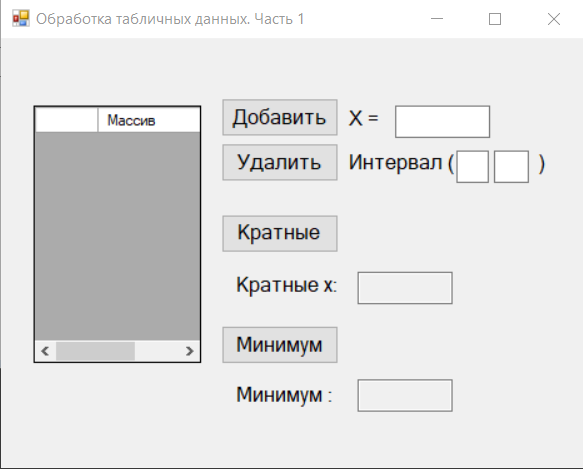
\includegraphics[width=0.6\linewidth]{lections/img/task4_launch1.png}
    \caption{Запуск программы}
    \label{task4_launch1}
\end{figure}


При вводе целого X в поле ввода и нажатии на кнопку <<Добавить>> (на рисунке \ref{task4_launch2}).
\begin{figure}[H]
    \centering
    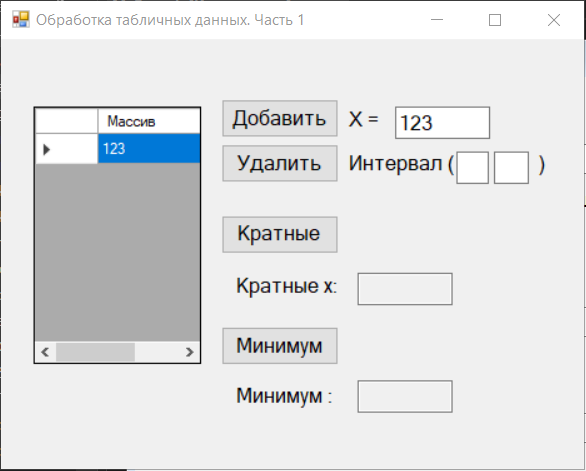
\includegraphics[width=0.6\linewidth]{lections/img/task4_launch2.png}
    \caption{Вычисление выражения}
    \label{task4_launch2}
\end{figure}

При попытке ввода не числа, программа выведет ошибку (на рисунке \ref{task4_launch3})
\begin{figure}[H]
    \centering
    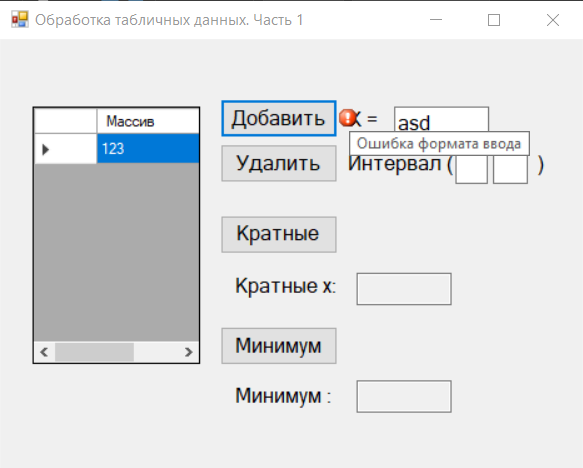
\includegraphics[width=0.7\linewidth]{lections/img/task4_launch3.png}
    \caption{Ошибка формата ввода}
    \label{task4_launch3}
\end{figure}

\subsection{Примеры исходного кода}


Функция при нажатии на кнопку "Кратные Х".
\begin{minted}[style=bw,
 linenos=true,
 breaklines=true,
 numbersep=5pt,
 tabsize=2,
 fontsize=\small,
 bgcolor=white]{cpp}
private: System::Void krat_btn_Click(System::Object^ sender, System::EventArgs^ e) {
	this->errorProvider1->Clear();
	this->krat_box->Text = "";
	long long x,y,a,b;
	bool result = Int64::TryParse(this->x_input->Text, x);
	bool resulta = Int64::TryParse(this->int_a->Text, a);
	bool resultb = Int64::TryParse(this->int_b->Text, b);
	if (!result) {
		this->errorProvider1->SetError(this->x_input, "Неправильный формат числа X");
		return;
	}
	if (!resulta || !resultb) {
		this->errorProvider1->SetError(this->int_a, "Неправильный формат границ интервала");
		return;
	}
	bool found_krat = false;
	for (int i = a; i < this->mas_grid->RowCount && i < b; i++) {
		result = Int64::TryParse(this->mas_grid->Rows[i]->Cells[0]->Value->ToString(), y);
		if (y % x == 0) {
			found_krat = true;
			this->krat_box->Text += System::Convert::ToString(i+1) + ", ";
		}
	}
	if (!found_krat) {
		this->krat_box->Text = "Таких элементов нет";
	}
}
\end{minted}
Другие фрагменты кода расположены в приложении \ref{app:table_data}.
\sectionbreak